
\documentclass[12pt]{article}


\usepackage{cite}
\usepackage{graphicx}
\usepackage{subfigure}
\usepackage{epsfig}
\usepackage{epstopdf}
\usepackage{subfigure}
\usepackage{calc}
\usepackage{amssymb}
\usepackage{amstext}
\usepackage[fleqn]{amsmath}


\title{VelaLab reference Manual}

%\author{
%        Vitaly Surazhsky \\
%                Department of Computer Science\\
%        Technion---Israel Institute of Technology\\
%        Technion City, Haifa 32000, \underline{Israel}
%            \and
%        Yossi Gil\\
%        Department of Computer Science\\
%        Technion---Israel Institute of Technology\\
%        Technion City, Haifa 32000, \underline{Israel}
%}

\date{\today}


\begin{document}
\maketitle

%\begin{abstract}
%This is the paper's abstract \ldots
%\end{abstract}



\section{System Architecture}

Figure of the system... 

\begin{figure}[h]
	\centering
	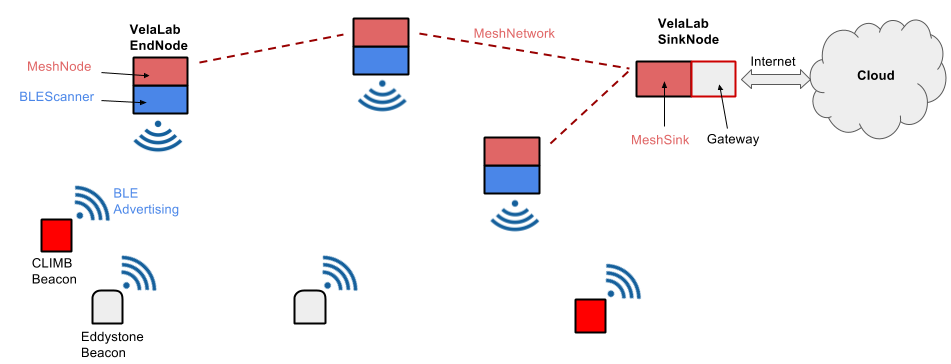
\includegraphics[width=0.98\columnwidth]{fig/Architecture.png}
	\caption{}
	\label{fig:system}
\end{figure}



\subsection{Namings and conventions}

Names of all the different boards and devices...


\section{Beacons}

Types:
\begin{itemize}
\item{CLIMB (custom)}
\item{Eddystone}
\end{itemize}




\section{VelaLab End-Node}

Components:
\begin{itemize}
\item{BLE Scanner}
\item{Mesh Node}
\end{itemize}



\subsection{Hardware interconnection}

fig...

\begin{figure}[!h]
	\centering
	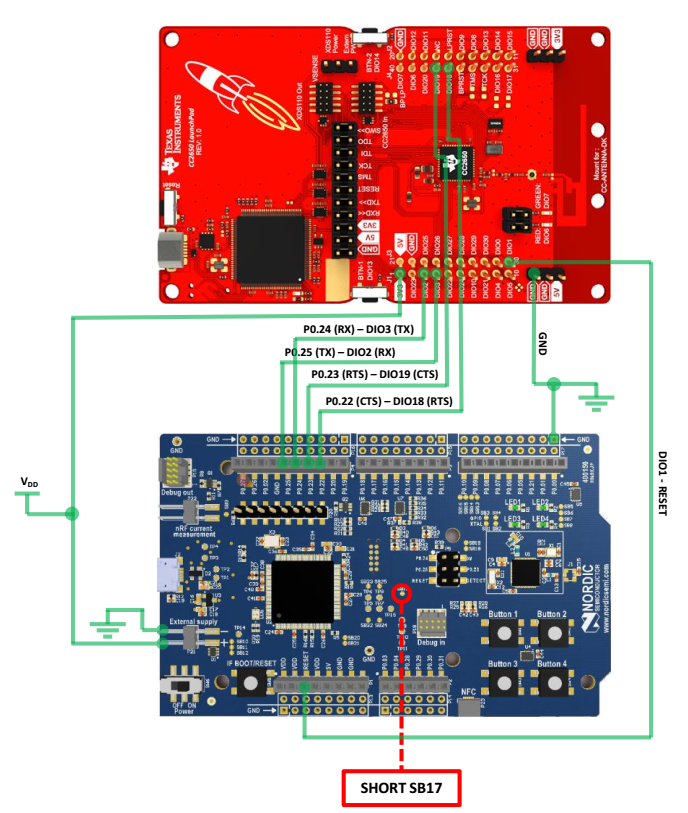
\includegraphics[width=0.7\columnwidth]{fig/VelaNode_hw.png}
	\caption{}
	\label{fig:system}
\end{figure}

The Launchpad image refers to the revision 1.0 of the hardware. In that version the DIO2 and DIO3 pins were incorrectly labelled (labels are swapped with respect to actual pin location). This scheme refers to the actual wiring position, then discard any label on the board and just wire as shown.


\subsection{Communication protocol}

UART communication protocol between BLE Scanner and Mesh Node


\section{VelaLab Sink-Node}

Components:
\begin{itemize}
\item{Mesh Sink}
\item{Gateway}
\end{itemize}

\subsection{Hardware interconnection}


Launchpad usb output to RPI's USB


\subsection{Communication protocol}


UART communication protocol between Mesh Sink and Gateway







%\bibliographystyle{abbrv}
%\bibliography{main}

\end{document}
This is never printed